\begin{frame}
    \frametitle{M\'etodo de vol\'umenes finitos}
    \framesubtitle{Condiciones de borde}

    \begin{columns}

      \column{0.5\textwidth}
      \begin{figure}[h]
        \begin{center}
          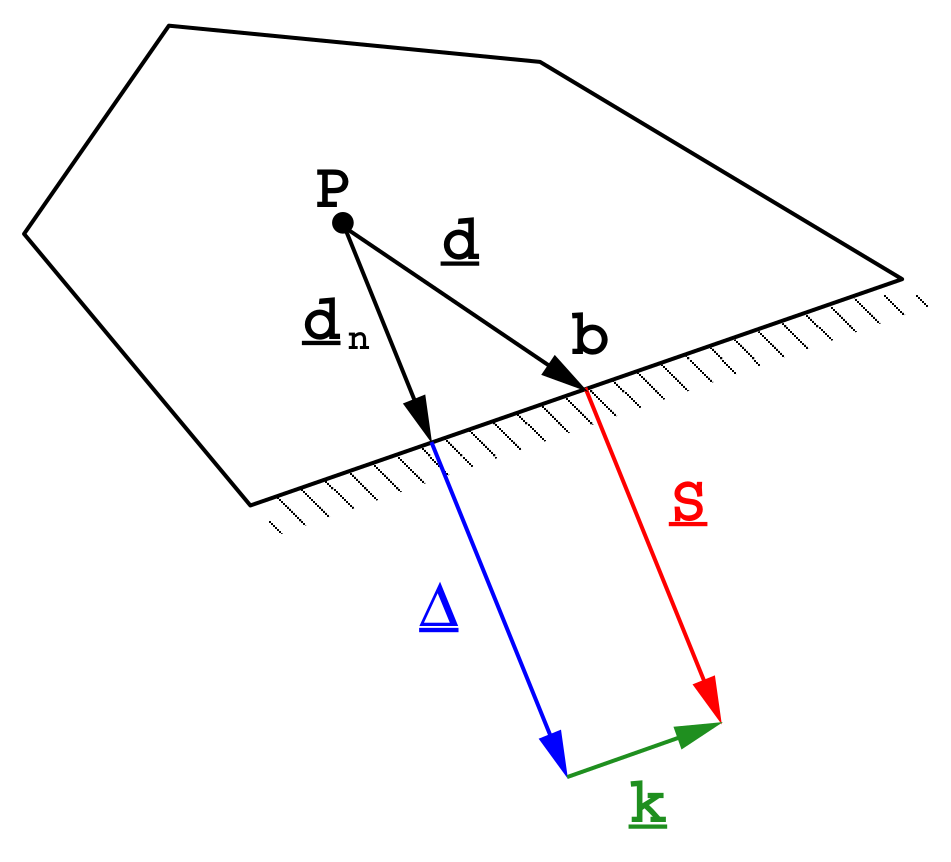
\includegraphics[width = \textwidth]{Imagenes/BC}
        \end{center}
      \end{figure}


      \column{0.45\textwidth}
      La condici\'on se extiende a toda la cara. La componente ortogonal es igual a $\bs{S}$, pero no se encuentra en el centro de la cara. El vector entre el centro de celda y la cara es normal a la frontera

      $$ \bs{d_n} = \frac{\bs{S}}{|\bs{S}|} \frac{\bs{d} \cdot \bs{S}}{|\bs{S}|} $$

      y ya no se emplea la correcci\'on $\bs{k}$

    \end{columns}

\end{frame}



\begin{frame}
    \frametitle{M\'etodo de vol\'umenes finitos}
    \framesubtitle{Condiciones de borde}

    \textbf{Valor fijo (Dirichlet)}

    El valor de $\phi$ en la cara $b$ es $\phi_b$.

    \begin{itemize}

    \item \textbf{T\'ermino convectivo}

      $$ \int_{V_{P}} \nabla \cdot (\rho \bs{U} \phi) dV = \sum_f F \phi_f $$
      
    \item \textbf{T\'ermino difusivo}

      $$ \int_{V_{P}} \nabla \cdot (\rho \Gamma_{\phi} \nabla \phi) dV = \sum_f (\rho \Gamma_{\phi})_f \bs{S} \cdot (\nabla \phi)_f = \sum_f (\rho \Gamma_{\phi})_f |\bs{S}| \frac{\phi_b - \phi_P}{|\bs{d_n}|} $$
      
    \end{itemize}

\end{frame}




\begin{frame}
    \frametitle{M\'etodo de vol\'umenes finitos}
    \framesubtitle{Condiciones de borde}

    \textbf{Gradiente fijo (Newmann)}

    Queda determinado el producto interno entre el gradiente y la normal
    $$ \left ( \frac{\bs{S}}{|\bs{S}|} \cdot \nabla \phi \right )_b = g_b$$

    \begin{itemize}

    \item \textbf{T\'ermino convectivo}

      $$ \phi_b = \phi_P + \bs{d_n} \cdot (\nabla \phi)_b = \phi_P + |\bs{d_n}| g_b $$
      
    \item \textbf{T\'ermino difusivo}

      Para el t\'ermino correspondiente se emplea
      $$ (\rho \Gamma_{\phi})_b |\bs{S}| g_b $$
      
    \end{itemize}

\end{frame}
